\documentclass[conference]{IEEEtran}
\IEEEoverridecommandlockouts
\usepackage{cite}
\usepackage{amsmath,amssymb}
\usepackage{graphicx}
\usepackage{booktabs}
\usepackage{url}
\usepackage{tikz}
\usetikzlibrary{positioning,arrows.meta,calc}

% Every claim and number below is listed in _claims.md with its evidence.

\begin{document}

\title{Real-Time Digital Hearing Aid using Multirate Filter Bank and FFT-Based Overlap-Add Processing on TMS320C6748}

\author{\IEEEauthorblockN{Aneesh Venkatesha Rao, Akula Sahasra, Adhvay Shrujal}
\IEEEauthorblockA{\textit{Department of Electronics and Communication Engineering}\\
\textit{National Institute of Technology Warangal}, Warangal, India\\
\{TODO-email-1, TODO-email-2, TODO-email-3\}}}

\maketitle

\begin{abstract}
Hearing loss varies with frequency, so a hearing aid must apply a different gain in each band while adding little delay. This paper reports the real-time implementation and evaluation of two equalisers on a Texas Instruments TMS320C6748 digital signal processor (DSP) at 48~kHz: a five-band complementary multirate octave filter bank (Mode~A) and a 129-tap frequency-sampling finite impulse response (FIR) filter applied by fast Fourier transform (FFT) overlap-add with a 256-point FFT (Mode~B). Gains follow the half-gain rule on the Bisgaard N3 standard audiogram with a 30~dB cap. On the board, the DSP output matches a floating-point reference within $2.0\times10^{-5}$ of full scale, and band gains measured on the DSP match the design within 0.01~dB. The measured processor load with the codec running is 10.5\,\% (Mode~A) and 4.2\,\% (Mode~B) at 300~MHz. The calculated input-to-output latency is 8.81~ms and 7.67~ms. In simulation, Mode~A follows the N3 prescription within 1.53~dB and Mode~B within 0.38~dB; for the steep S2 audiogram the errors are 6.82~dB and 0.49~dB, so five octave bands are unsuitable for steep losses. Latency was not measured on the board.
\end{abstract}

\begin{IEEEkeywords}
hearing aids, multirate filter banks, overlap-add, FFT, real-time DSP, TMS320C6748
\end{IEEEkeywords}

% =====================================================================
\section{Introduction}
Sensorineural hearing loss (damage to the inner ear or auditory nerve) is described by an audiogram, the hearing threshold in dB hearing level (dB~HL) at audiometric frequencies from 250~Hz to 8~kHz. Typical standard audiograms show a loss that grows with frequency~\cite{bisgaard2010}, so a hearing aid must apply frequency-dependent gain that follows the audiogram. A second constraint is delay: the wearer hears both the processed sound and the direct sound leaking past the device, and a long processing delay causes comb filtering and an audible echo. Published hearing-aid work uses about 10~ms as the upper limit~\cite{sokolova2021,kayser2022,yang2016}.

Real-time designs reported in the literature use either multirate filter banks~\cite{sokolova2021,sokolova2022,yang2016} or block processing based on the fast Fourier transform (FFT)~\cite{kayser2022}. This paper does not propose a new algorithm. It is an implementation and evaluation study that builds both approaches on the same embedded processor so that they can be compared on equal terms. The contributions are:
\begin{enumerate}
\item a real-time implementation on the TMS320C6748 of a five-band complementary multirate octave filter bank (Mode~A) and of an FFT overlap-add (OLA) equaliser with a frequency-sampling finite impulse response (FIR) filter (Mode~B), switchable at run time;
\item board measurements of numerical agreement with a reference model, band gains and processor load, together with a calculated latency budget for both modes;
\item an evaluation of prescription accuracy on three standard audiograms (N2, N3, S2), showing quantitatively that five octave bands cannot follow a steep loss while the 129-tap FIR can;
\item a staged verification flow (Python reference, MATLAB, portable C on a PC, C on the DSP) with pre-declared tolerances, and a record of the board-only defects it exposed.
\end{enumerate}
Section~\ref{sec:bg} reviews related work, Section~\ref{sec:design} describes the design, Section~\ref{sec:impl} the implementation, Section~\ref{sec:results} the results and Section~\ref{sec:disc} discusses trade-offs and limitations.

% =====================================================================
\section{Background and Related Work}\label{sec:bg}
\subsection{Multirate audiometric filter banks}
Sokolova et~al.~\cite{sokolova2021} designed a ten-band audiometric filter bank from complementary filters, so that the bands sum to an all-pass, and implemented the resampling with cascaded 2:1 half-band stages. They report a 9.1-fold reduction in operations over a single-rate bank, and show that the bands must be delay-aligned to avoid audible distortion of the summed response. Their 11-band half-octave system~\cite{sokolova2022,garudadri2026patent} reports a 13.67-fold saving and a latency of about 32~ms with linear-phase filters, reduced to 5.4~ms with minimum-phase filters. Garudadri et~al.~\cite{garudadri2017} describe an open real-time research platform with a 7.98~ms latency.

\subsection{ANSI S1.11 filter-bank specifications}
Yang et~al.~\cite{yang2016} relate filter-bank design to the American National Standards Institute (ANSI) S1.11 class-2 limits (passband ripple within $\pm0.5$~dB, stopband attenuation above 60~dB) and relax the specification to meet a delay target of about 10~ms. Their path-delay formula (eq.~(15) in~\cite{yang2016}) is used to check our delay in Section~\ref{sec:modea}. We did not read the ANSI standard itself or the listening studies on tolerable delay; these are known to us only through~\cite{yang2016,sokolova2021}.

\subsection{Compression and FFT processing}
Real hearing aids add wide dynamic range compression (WDRC). Sokolova et~al.~\cite{sokolova2022,garudadri2026patent} give an automatic gain control loop with attack and release coefficients, and Kates~\cite{kates2005} discusses the trade-offs between filter-bank and FFT-based compressors in frequency resolution, delay and complexity. The open Master Hearing Aid~\cite{kayser2022} processes audio by FFT overlap-add. WDRC was not built in this work.

\subsection{Audiograms and gain rules}
Bisgaard et~al.~\cite{bisgaard2010} define standard audiograms for hearing-aid measurement. We use the moderate N3 audiogram as the default, the mild N2, and the mild but steeply sloping S2 as a stress case. Their tables stop at 6~kHz; no 8~kHz value was extrapolated. The gain rule is the half-gain rule (gain equal to half the hearing loss), attributed to Lybarger and cited here through Venema~\cite{venema2001}, the source we read.

% =====================================================================
\section{System Design}\label{sec:design}
Fig.~\ref{fig:block} shows the signal chain. The sample rate is 48~kHz, so that the octave crossovers $f_s/8$, $f_s/16$, $f_s/32$ and $f_s/64$ fall at 6~kHz, 3~kHz, 1.5~kHz and 750~Hz.

\begin{figure}[t]
\centering
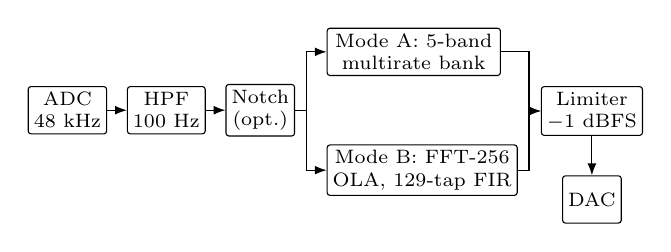
\begin{tikzpicture}[font=\scriptsize, node distance=3mm and 2.5mm,
  blk/.style={draw, rounded corners=1pt, align=center, minimum height=6mm, inner sep=2pt},
  ar/.style={-{Latex[length=1.5mm]}}]
\node[blk] (adc) {ADC\\48 kHz};
\node[blk, right=of adc] (hpf) {HPF\\100 Hz};
\node[blk, right=of hpf] (nt) {Notch\\(opt.)};
\node[blk, minimum width=22mm, above right=1mm and 4mm of nt] (a) {Mode A: 5-band\\multirate bank};
\node[blk, minimum width=22mm, below right=1mm and 4mm of nt] (b) {Mode B: FFT-256\\OLA, 129-tap FIR};
\node[blk, anchor=west] (lim) at ($(a.east)!0.5!(b.east)+(4mm,0)$) {Limiter\\$-1$ dBFS};
\node[blk, below=5mm of lim] (dac) {DAC};
\draw[ar] (adc) -- (hpf);
\draw[ar] (hpf) -- (nt);
\draw[ar] (nt.east) -- ++(1.5mm,0) |- (a.west);
\draw[ar] (nt.east) -- ++(1.5mm,0) |- (b.west);
\draw[ar] (a.east) -| ([xshift=-1.5mm]lim.west) -- (lim.west);
\draw[ar] (b.east) -| ([xshift=-1.5mm]lim.west) -- (lim.west);
\draw[ar] (lim) -- (dac);
\end{tikzpicture}
\caption{Signal chain. The AIC3106 codec provides the analogue-to-digital converter (ADC) and digital-to-analogue converter (DAC). The notch and noise suppression are optional and off by default.}
\label{fig:block}
\end{figure}

\subsection{Input high-pass filter}
A fourth-order Butterworth high-pass filter (HPF) at 100~Hz removes direct current (DC) offset and low-frequency rumble. It was designed by the bilinear transform with pre-warping and realised as two second-order sections in direct form~II transposed (DF-II-T); the simulated response at 100~Hz is $-3.01$~dB. Impulse invariance is not applicable to a high-pass filter because the analogue impulse response contains a delta and the design aliases.

\subsection{Mode A: five-band multirate octave bank}\label{sec:modea}
Each of four levels $k=0,\dots,3$ runs at $f_{s,k}=48/2^k$~kHz. A 21-tap Kaiser-window low-pass filter $G$ ($\beta=4.5$, cut-off $f_{s,k}/8$) precedes decimation by two, and a 31-tap half-band filter $F$ (17 non-zero taps, centre tap 0.5) interpolates the output of the lower levels back up by two. The high band of each level is the delayed input minus the low-pass path, so the bank is complementary: with unity gains the output is the input delayed by 375 samples, with a simulated ripple of $+0.020/-0.010$~dB (Fig.~\ref{fig:bands}). Filter lengths follow the Kaiser estimate~\eqref{eq:kaiser}~\cite{proakis2007}
\begin{equation}
N \approx \frac{A-7.95}{14.36\,\Delta f}+1, \label{eq:kaiser}
\end{equation}
where $A$ is the stopband attenuation in dB and $\Delta f$ the normalised transition width. With $A=50$~dB, $\Delta f=0.15$ gives 21 taps for $G$ and $\Delta f=0.10$ gives 31 for $F$ (half-band lengths are $4m-1$). The achieved stopbands are 52.5~dB ($G$) and 51.1~dB ($F$). Because $G$ is already 52~dB down at $0.20f_{s,k}$, and decimation folds $0.30$--$0.50f_{s,k}$ onto $0$--$0.20f_{s,k}$, the simulated alias rejection is $-73.4$~dB per level and the image rejection $-74.4$~dB.

The path delay at level $k$, in samples at that level's rate, is
\begin{equation}
T_k = \frac{N_G-1}{2}+\frac{N_F-1}{2}+2T_{k+1} = 10+15+2T_{k+1}, \quad T_4=0, \label{eq:delay}
\end{equation}
so $T_0 = 25(2^4-1)=375$ samples, or 7.81~ms. This equals eq.~(15) of~\cite{yang2016} applied to the deepest path, and the simulated impulse response peaks at sample 375. The lowest level alone contributes 4.17~ms. Alignment delays of 365, 165, 65 and 15 samples keep the bands in phase. The bank needs 61 operations per input sample against 313 for a single-rate bank with the same transition widths, a calculated saving of 5.1 times.

\begin{figure}[t]
\centering
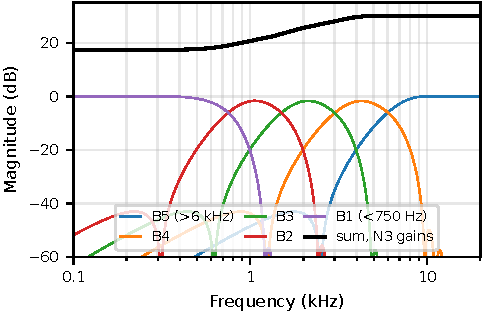
\includegraphics[width=\columnwidth]{figures/fig_bands.pdf}
\caption{Mode~A (simulated): magnitude response of each band with unity gain, and of the sum with the N3 half-gain band gains of Table~\ref{tab:gains}.}
\label{fig:bands}
\end{figure}

\subsection{Mode B: FFT overlap-add}
The same prescription is realised as a linear-phase FIR of length $M=129$ by frequency sampling: the gain is specified at 65 frequencies $k f_s/129$, a 372~Hz grid. This design follows the N3 target within 0.38~dB in simulation, against 1.00~dB for a Kaiser-window design of the same length. The filter is applied by overlap-add with $L=128$ new samples per block and an FFT size $N$ that satisfies the OLA condition
\begin{equation}
N \ge L+M-1 = 128+129-1 = 256, \label{eq:ola}
\end{equation}
so that, by~\eqref{eq:ola}, circular convolution equals linear convolution. In simulation, OLA and overlap-save both match direct convolution within $1.2\times10^{-14}$, while undersized transforms alias in time (errors 0.29, 9.5 and 18.9 at $N=224$, 192 and 160). The processing delay is modelled as
\begin{equation}
D_B = 2L+\frac{M-1}{2} = 320 \text{ samples} = 6.67\ \text{ms}, \label{eq:delayB}
\end{equation}
one block filling, one block playing out, and the FIR group delay. This buffering model is an assumption.

\subsection{Gain prescription and limiter}
The band gain is
\begin{equation}
g_b = \min\!\left(0.5\,\mathrm{HL}(f_b),\ 30\ \mathrm{dB}\right), \label{eq:gain}
\end{equation}
where $\mathrm{HL}(f_b)$ is the N3 hearing level interpolated on a logarithmic frequency axis at a representative frequency $f_b$ of each band (the geometric centre for B2--B4, the mean of the 250--500~Hz values for B1, and the 6~kHz value for B5). Table~\ref{tab:gains} lists the result of~\eqref{eq:gain} for N3. The 30~dB cap is a design choice that limits feedback and clipping on the bench. A hard limiter holds the output at $-1$~dB relative to full scale (dBFS); with speech at a root-mean-square (RMS) level of $-40$~dBFS and up to 30~dB of gain, 0.04\,\% of samples reach it in Mode~A and 0.03\,\% in Mode~B (simulated). Button S3 also selects N2, S2 and a bypass preset.

\begin{table}[t]
\centering
\caption{Mode A bands and N3 half-gain band gains (calculated)}
\label{tab:gains}
\begin{tabular}{@{}llrr@{}}
\toprule
Band & Range & Rate (kHz) & Gain (dB) \\
\midrule
B5 & $>6$ kHz & 48 & 30.00 \\
B4 & 3--6 kHz & 24 & 30.00 \\
B3 & 1.5--3 kHz & 12 & 25.36 \\
B2 & 0.75--1.5 kHz & 6 & 20.36 \\
B1 & $<750$ Hz & 3 & 17.50 \\
\bottomrule
\end{tabular}
\end{table}

\subsection{Optional extras}
Two optional blocks, off by default, were added: a second-order notch obtained by the bilinear transform of $H(s)=(s^2+\omega_0^2)/(s^2+(\omega_0/Q)s+\omega_0^2)$ with $Q=10$, placed automatically by a howl detector (a stable spectral peak at least 25~dB above the mean of 500~Hz--8~kHz in a Hann-windowed 256-point FFT, confirmed by a leaky counter reaching 75 blocks), and a noise suppressor (noise reduction, NR) with gain $\sqrt{\max(1-2N/P,\,G_{\min}^2)}$, $G_{\min}=-12$~dB, using a simplified minimum-statistics noise estimate. These are standard methods; their primary sources were not consulted, and all parameters are our choices.

% =====================================================================
\section{Implementation on the TMS320C6748}\label{sec:impl}
\subsection{Platform and audio input/output (I/O)}
The target is the Texas Instruments (TI) low-cost development kit (LCDK)~\cite{ti_spruil2} with a TMS320C6748 digital signal processor (DSP), whose C674x very long instruction word (VLIW) core has eight functional units and hardware floating point~\cite{ti_sprs590,ti_sprufe8}. The central processing unit (CPU) clock is 300~MHz, confirmed on the board from the phase-locked loop (PLL) registers ($24~\mathrm{MHz}\times25/2$)~\cite{ti_spruh79} and from the time-stamp counter (TSCL) against a PC timer, which gives exactly 6250.0 cycles per sample. The TLV320AIC3106 codec~\cite{ti_slas509} is configured over the inter-integrated circuit (I$^2$C) bus as clock master in DSP mode, 16~bits at 48~kHz, using the board-support code of~\cite{welch2017}. The multichannel audio serial port (McASP)~\cite{ti_sprufm1} runs with its read first-in first-out (FIFO) buffer enabled (four words) and its write FIFO disabled; the enhanced direct memory access (EDMA3) controller moves four-sample blocks, producing one interrupt every 83.3~$\mu$s, a budget of 25\,000 cycles. Enabling the write FIFO would add 64 samples (1.33~ms) and push the calculated Mode~A latency to 10.15~ms. On the board, the read FIFO produced one interrupt per four samples at 104 cycles per interrupt, with no McASP errors.

\subsection{Processing code}
Mode~A runs per sample in plain C. The block routines of the C674x DSP library (DSPLIB)~\cite{ti_dsplib674} need multi-sample blocks and cannot be called per sample. Each level keeps a power-of-two circular history (512/256/128/16 samples) indexed with a mask. Mode~B fills a 128-sample buffer in the interrupt while a background loop processes the previous block (double buffering) with \texttt{DSPF\_sp\_fftSPxSP} and \texttt{DSPF\_sp\_ifftSPxSP}. All arithmetic is single-precision floating point, chosen because in simulation the float32 path reaches 85.0~dB (HPF), 138.7~dB (Mode~A) and 139.5~dB (Mode~B) signal-to-noise ratio (SNR) against float64, compared with 12.1, 42.7 and 20.2~dB for 16-bit Q15 fixed point. The HPF state is kept in double precision: with poles at radius 0.995, float32 state produced errors of $3.9\times10^{-5}$ that the 30~dB band gains amplified past the chain tolerance. The program occupies 22.1~KB of code and 68.6~KB of the 256~KB L2 memory; large test buffers sit in external DDR2.

\subsection{Verification flow}
A Python model is the reference for every block. MATLAB versions reproduce it, and the portable C is compiled on a PC and fed the same test vectors (C against Python: at most $2.2\times10^{-5}$ for full chains). On the board, a mode without the codec processes a stored test signal and its output is read back over the Joint Test Action Group (JTAG) debug interface and compared sample by sample. Tolerances were fixed before testing: $10^{-5}$ of full scale for single blocks, $10^{-4}$ for chains, and 0.05~dB for tone gains. Cycle counts come from TSCL, and all board runs were scripted with the Code Composer Studio debug server so that they could be repeated.

% =====================================================================
\section{Results}\label{sec:results}
Values in this section are labelled \emph{measured} (on the board), \emph{simulated} (PC) or \emph{calculated} (model).

\subsection{Numerical agreement and band gains (measured)}
The DSP processed a stored signal of 11 tones at $-40$~dBFS followed by noise. The maximum deviation of its output from the Python reference is $6.1\times10^{-6}$ of full scale in both modes and $2.0\times10^{-5}$ ($9.4\times10^{-6}$) in Mode~A (Mode~B) with noise suppression, all within the $10^{-4}$ tolerance. A Goertzel tone meter running on the DSP ($N=4608$, so that every test tone falls on a bin) measured the gains in Table~\ref{tab:tones}; they equal the simulated design within 0.01~dB (Fig.~\ref{fig:boardgains}). Mode~A deviates most from the target at the 750~Hz crossover (1.53~dB), as the design predicts; at the test tones Mode~B stays within 0.33~dB of the target.

\begin{table}[t]
\centering
\caption{Band gains measured on the DSP, N3 preset (dB)}
\label{tab:tones}
\begin{tabular}{@{}rrrr@{}}
\toprule
Frequency (Hz) & Target & Mode A & Mode B \\
\midrule
250 & 17.5 & 17.40 & 17.59 \\
375 & 17.5 & 17.41 & 17.50 \\
500 & 17.5 & 17.65 & 17.27 \\
750 & 17.5 & 19.03 & 17.53 \\
1000 & 20.0 & 20.66 & 19.67 \\
1500 & 22.5 & 23.33 & 22.50 \\
2000 & 25.0 & 25.60 & 25.00 \\
3000 & 27.5 & 28.02 & 27.50 \\
4000 & 30.0 & 29.66 & 29.89 \\
6000 & 30.0 & 30.00 & 29.99 \\
8000 & 30.0 & 30.00 & 30.02 \\
\bottomrule
\end{tabular}
\end{table}

\begin{figure}[t]
\centering
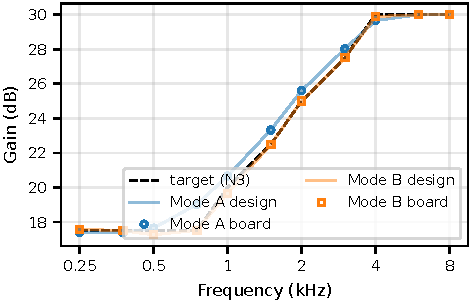
\includegraphics[width=\columnwidth]{figures/fig_board_gains.pdf}
\caption{Band gains measured on the DSP (markers) against the simulated design (lines) and the N3 half-gain target.}
\label{fig:boardgains}
\end{figure}

\subsection{Prescription accuracy on three audiograms (simulated)}
Table~\ref{tab:acc} and Fig.~\ref{fig:acc} compare both modes with the target over 250~Hz--8~kHz. For the mild and moderate audiograms both modes stay within the 3~dB just-noticeable criterion used in~\cite{sokolova2021,sokolova2022}. For the steep S2 audiogram the target rises by 15.73~dB between adjacent bands B2 and B3; the octave-wide bands of Mode~A cannot follow this and overshoot by 6.82~dB at 1.5~kHz, while the 372~Hz grid of Mode~B follows within 0.49~dB.

\begin{table}[t]
\centering
\caption{Maximum gain error against the half-gain target, 250~Hz--8~kHz (simulated, dB)}
\label{tab:acc}
\footnotesize
\begin{tabular}{@{}lrrr@{}}
\toprule
Audiogram & Max.\ step, adjacent bands & Mode A & Mode B \\
\midrule
N2 (mild) & 5.00 & 1.01 & 0.22 \\
N3 (moderate) & 5.00 & 1.53 & 0.38 \\
S2 (steep) & 15.73 & 6.82 & 0.49 \\
\bottomrule
\end{tabular}
\end{table}

\begin{figure}[t]
\centering
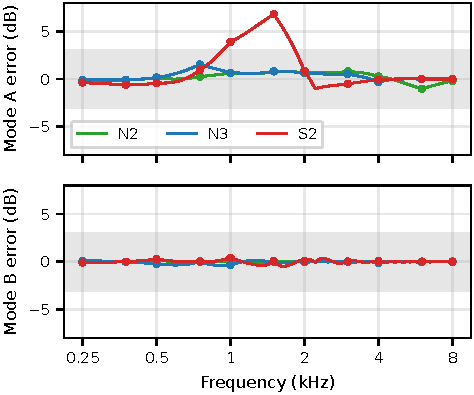
\includegraphics[width=\columnwidth]{figures/fig_accuracy.pdf}
\caption{Gain error against the target for N2, N3 and S2 (simulated); markers at the 11 test tones. The shaded band is $\pm3$~dB.}
\label{fig:acc}
\end{figure}

\subsection{Latency (calculated)}
Fig.~\ref{fig:lat} breaks down the latency. Mode~A adds the 375-sample bank delay of~\eqref{eq:delay}, Mode~B the 320 samples of~\eqref{eq:delayB}; both add an assumed 10 samples (0.21~ms) of FIFO and block buffering, and the codec's 17-sample ADC and 21-sample DAC group delays from its data sheet~\cite{ti_slas509} (0.79~ms). The totals are 8.81~ms and 7.67~ms, both under 10~ms. These values were \emph{not} measured on the board (Section~\ref{sec:threats}); in the PC C build, the Mode~B buffering delay is exactly 256 samples, as modelled.

\begin{figure}[t]
\centering
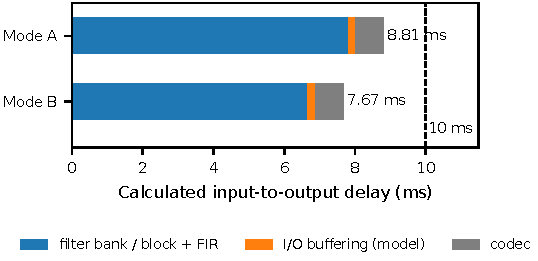
\includegraphics[width=\columnwidth]{figures/fig_latency.pdf}
\caption{Calculated input-to-output latency. The I/O buffering term is a model assumption.}
\label{fig:lat}
\end{figure}

\subsection{Processor load and cycle counts (measured)}
Table~\ref{tab:cpu} gives the cycle counts over 60~s per mode with the codec running. Mode~A uses 10.5\,\% of the CPU (11.1\,\% in the worst block) and Mode~B 4.2\,\%, with no overruns, no McASP errors and no limiting. The estimates made before board testing were 2.5--10.2\,\% and 2.6--5.0\,\%: Mode~B falls inside its range and Mode~A slightly above it. Without the codec, noise suppression raises the load to 25.1\,\% (Mode~A) and 12.0\,\% (Mode~B). Mode~B is cheaper because two library FFTs per 128 samples cost less than four levels of per-sample filtering in C.

\begin{table}[t]
\centering
\caption{Cycle counts and load on the DSP at 300~MHz (measured)}
\label{tab:cpu}
\footnotesize
\setlength{\tabcolsep}{3pt}
\begin{tabular}{@{}lrr@{}}
\toprule
Quantity & Mode A & Mode B \\
\midrule
Interrupt per 4 samples (avg/max) & 2617 / 2785 & 829 / 851 \\
Background per 128 samples (avg/max) & --- & 7242 / 7253 \\
CPU load, live (avg) & 10.5\,\% & 4.2\,\% \\
Load, no codec, without / with NR & 10.1 / 25.1\,\% & 3.8 / 12.0\,\% \\
\midrule
\multicolumn{3}{@{}l}{Benchmarks (cycles)} \\
DFT-256: direct / own FFT / DSPLIB & \multicolumn{2}{r}{107\,797\,012 / 228\,676 / 2145} \\
21-tap FIR $\times$48: DSPLIB / C \texttt{-O3} / C \texttt{-O0} & \multicolumn{2}{r}{838 / 1052 / 25\,402} \\
256-term MAC: int16 / int32 / float / double & \multicolumn{2}{r}{316 / 522 / 326 / 1000} \\
\bottomrule
\end{tabular}
\end{table}

The benchmarks illustrate the architecture. The library FFT is about 50\,000 times faster than a direct discrete Fourier transform (DFT); our textbook radix-2 FFT computes its twiddle factors with double-precision trigonometry inside the loop and is about 100 times slower than the library. Compiler optimisation (\texttt{-O3} against \texttt{-O0}) speeds up the plain-C FIR loop 24 times and the complete modes 3.0 (Mode~A) and 3.6 times (Mode~B). A float multiply-accumulate (MAC) costs about the same as an int16 MAC, which, with the SNR results of Section~\ref{sec:impl}, supports the float32 choice.

\subsection{Optional extras (measured with built-in signals)}
With a 2~s built-in speech clip and on-board white noise at 5~dB SNR, noise suppression improved the SNR by 8.39~dB (Mode~A) and 8.78~dB (Mode~B); the speech level fell by 1.93 and 1.56~dB and the noise by 10.33 and 10.34~dB, and the board output equals the Python reference within $2\times10^{-5}$. In simulation on two voices with white and pink noise at 0--10~dB SNR, the improvement was 5.9--8.5~dB (Mode~A) and 6.5--9.4~dB (Mode~B). The automatic notch placed no notch on 12~s of speech. With a steady 2500~Hz tone 10~dB above the speech it placed one notch within 0.5~s, at 2500.48--2500.83~Hz over repeated runs (error at most 0.03\,\%). A tone at the speech level was deliberately not notched within 16~s, since the detector requires a 25~dB peak; the detection threshold between these levels was not measured.

% =====================================================================
\section{Discussion}\label{sec:disc}
\subsection{Mode A versus Mode B}
Mode~B is more accurate (0.38 against 1.53~dB on N3), handles steep losses, uses less than half the processor time and has a slightly lower calculated latency. Mode~A has no block structure: it processes each sample as it arrives, and its explicit bands are the natural place for per-band compression. Its processor cost comes from running $G$ and $F$ per sample in C at four rates; a block-based version using library FIR routines is estimated at about 2\,\% load but was not built. Mode~A's steep-loss error is structural: five octave bands change gain only in octave steps and blend neighbours near each crossover. The half-octave layout of~\cite{sokolova2022} would reduce it, but with linear-phase filters it exceeds our delay budget, since even a sixth octave band would raise the delay to about 16--17~ms.

\subsection{Stopband attenuation and delay}
The 52.5 and 51.1~dB stopbands fall short of the 60~dB of ANSI S1.11 class~2 as summarised in~\cite{yang2016}, while the unity-gain ripple of $+0.020/-0.010$~dB is well inside $\pm0.5$~dB. Reaching 60~dB with the same band edges requires 27 taps for $G$ and 39 for $F$, which raises the calculated latency to 10.79~ms. We kept 52~dB, the same kind of specification relaxation that~\cite{yang2016} argues for. The worst simulated crossover spur is $-68$~dB relative to the test tone (dBc). The full ANSI mask was not checked.

\subsection{Board-only defects}
Four defects appeared only on hardware: a clock estimate distorted by start-up overruns, a double write to the McASP at start-up, an interrupt race in the borrowed start-up code that stopped audio from starting after a power cycle, and an EDMA transfer left running by a previously loaded program that wrote into the new program's memory. Each was caught by the pre-declared checks rather than by listening, and all board measurements were repeated after the fixes.

\subsection{Threats to validity}\label{sec:threats}
No external audio input was used: the available PC could not drive the board's line input reliably, so the board was verified only with built-in signals. As a result, latency, analogue-path spurs and the limiter were not measured on the board, and the band gains exclude the codec's analogue response. Test speech was synthetic (text-to-speech), and there was no listener study, clinical evaluation or real-ear measurement; prescription accuracy is evaluated against the half-gain target only, not against a validated fitting rule. In an informal listening check of the board output, a 6~kHz test tone was not heard although its gain measures 30.00~dB on the DSP; the cause (codec, cable, transducer or level) was not determined. The noise-suppression and howl-detection methods were verified against our reference but not against published implementations.

% =====================================================================
\section{Conclusion and Future Work}
Both equalisers run in real time on the TMS320C6748 at 300~MHz with 10.5\,\% and 4.2\,\% processor load, match the reference model within $2.0\times10^{-5}$ and reproduce the designed band gains within 0.01~dB. The FFT overlap-add mode is more accurate, cheaper and better suited to steep losses; the multirate bank offers per-sample processing and explicit bands. Future work is to measure the end-to-end latency and analogue response with a live input, to add per-band WDRC, to evaluate minimum-phase filters, which~\cite{sokolova2022} shows can reduce delay but which change phase behaviour that~\cite{yang2016} cautions against, to add bands within the delay budget, and to evaluate the system with listeners.

\section*{Acknowledgment}
The authors thank TODO (faculty guide) and the DSP Laboratory of the Department of Electronics and Communication Engineering, National Institute of Technology Warangal.

\bibliographystyle{IEEEtran}
\bibliography{refs}

\end{document}
